\subsection{Modus Operandi}

\begin{frame}{Les tests}
	\begin{itemize}
		\item Définit la densité : $r = \frac{m}{n}$
	\end{itemize}
\end{frame}

\begin{frame}{Les tests}
	\begin{itemize}
		\item Définit la densité : $r = \frac{m}{n}$
		\item Fait varier le nombre de noeuds
	\end{itemize}
\end{frame}
\begin{frame}{Les tests}
	\begin{itemize}
		\item Définit la densité : $r = \frac{m}{n}$
		\item Fait varier le nombre de noeuds
		\item Réalise les trois algorithmes sur 100 graphes aléatoires différents
	\end{itemize}
\end{frame}
\begin{frame}{Les tests}
	\begin{itemize}
		\item Définit la densité : $r = \frac{m}{n}$
		\item Fait varier le nombre de noeuds
		\item Réalise les trois algorithmes sur 100 graphes aléatoires différents
		\item Trace les courbes
	\end{itemize}
\end{frame}

\subsection{Retour d'expériences}

\begin{frame}{Les résultats attendus}
	Pour une densité $r = O(n^2)$ : 
\end{frame}

\begin{frame}{Les résultats attendus}
	Pour une densité $r = O(n^2)$ : \begin{itemize}
		\item Une complexité en $O(n^4)$ pour Dinic
	\end{itemize}
\end{frame}

\begin{frame}{Les résultats attendus}
	Pour une densité $r = O(n^2)$ : \begin{itemize}
		\item Une complexité en $O(n^4)$ pour Dinic
		\item Une complexité en $O(n^3)$ pour les algorithmes FIFO et High Label
	\end{itemize}
\end{frame}

\begin{frame}{Les résultats attendus}
	Pour une densité $r = O(n^2)$ : \begin{itemize}
		\item Une complexité en $O(n^4)$ pour Dinic
		\item Une complexité en $O(n^3)$ pour les algorithmes FIFO et High Label
		\item Une exécution plus rapide pour FIFO et High Label
	\end{itemize}
\end{frame}

\begin{frame}{Les résultats obtenus}
	\begin{center}
	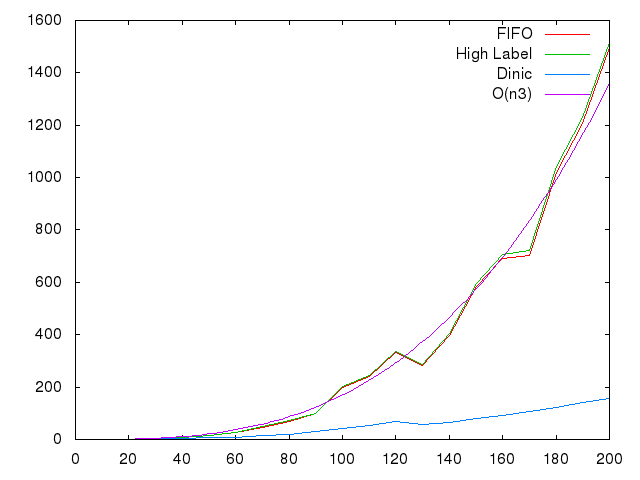
\includegraphics{img/resultat.png}
	\end{center}
\end{frame}


\begin{frame}{Les résultats obtenus}
	\begin{minipage}[c]{0.50\linewidth}
		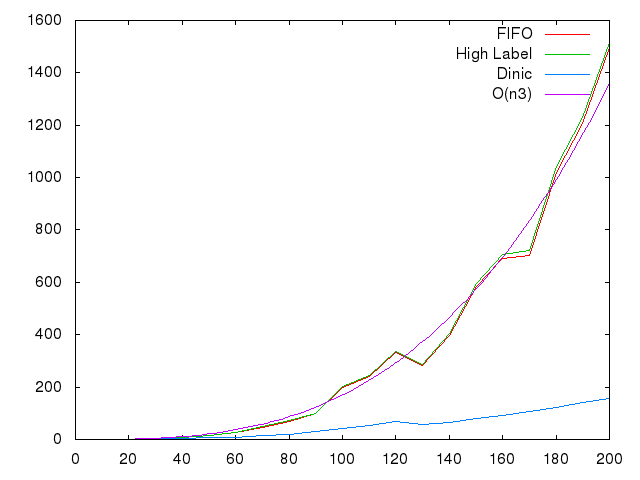
\includegraphics[scale=0.6]{img/resultat.png}
	\end{minipage}\hfill
	\begin{minipage}[c]{0.40\linewidth}
	\end{minipage}
\end{frame}

\begin{frame}{Les résultats obtenus}
	\begin{minipage}[c]{0.50\linewidth}
		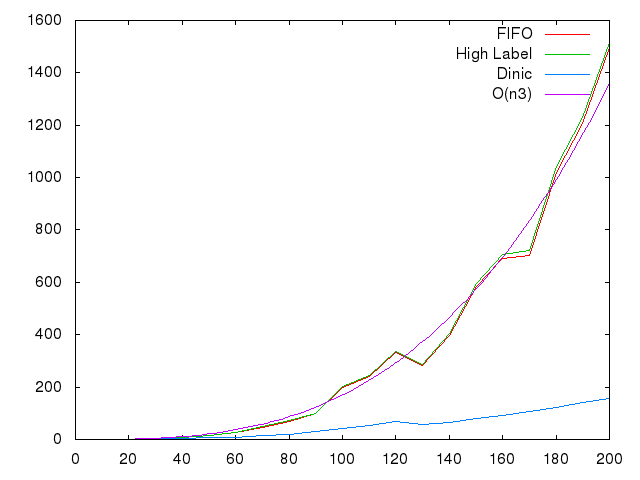
\includegraphics[scale=0.6]{img/resultat.png}
	\end{minipage}\hfill
	\begin{minipage}[c]{0.40\linewidth}
		\begin{itemize}
			\item $O(n^4)$ pour Dinic
			\end{itemize}
	\end{minipage}
\end{frame}

\begin{frame}{Les résultats obtenus}
	\begin{minipage}[c]{0.50\linewidth}
		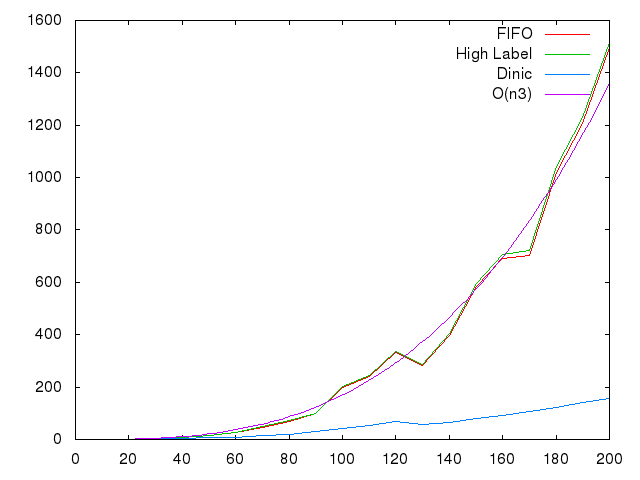
\includegraphics[scale=0.6]{img/resultat.png}
	\end{minipage}\hfill
	\begin{minipage}[c]{0.40\linewidth}
		\begin{itemize}
			\item $O(n^4)$ pour Dinic
			\item $O(n^3)$ pour les algorithmes de préflots
		\end{itemize}
	\end{minipage}
\end{frame}

\begin{frame}{Les résultats obtenus}
	\begin{minipage}[c]{0.50\linewidth}
		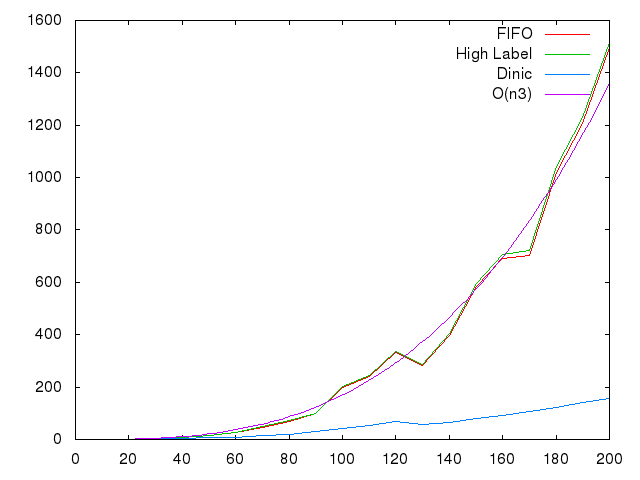
\includegraphics[scale=0.6]{img/resultat.png}
	\end{minipage}\hfill
	\begin{minipage}[c]{0.40\linewidth}
		\begin{itemize}
			\item $O(n^4)$ pour Dinic
			\item $O(n^3)$ pour les algorithmes de préflots
			\item Un temps égal pour les algorithmes de préflots
		\end{itemize}
	\end{minipage}
\end{frame}

